\documentclass[conference]{IEEEtran}
\IEEEoverridecommandlockouts
% The preceding line is only needed to identify funding in the first footnote. If that is unneeded, please comment it out.
%Template version as of 6/27/2024

\usepackage{cite}
\usepackage{amsmath,amssymb,amsfonts}
\usepackage{algorithmic}
\usepackage{graphicx}
\usepackage{textcomp}
\usepackage{xcolor}
\def\BibTeX{{\rm B\kern-.05em{\sc i\kern-.025em b}\kern-.08em
    T\kern-.1667em\lower.7ex\hbox{E}\kern-.125emX}}

\usepackage[hidelinks]{hyperref}

% numbers.tex — SỐ THẬT (5 seed, max-pool, test family-disjoint). 2026-09-30.
% Thay TOÀN BỘ numbers.tex hiện tại bằng file này.

% ---- H-GNN max-pool (mô hình chính), test 5 seed ----
\newcommand{\hgnnF}{97.99}
\newcommand{\hgnnFstd}{0.44}
\newcommand{\hgnnAcc}{97.69}
\newcommand{\hgnnAccStd}{0.51}
\newcommand{\hgnnPrec}{96.99}
\newcommand{\hgnnPrecStd}{1.06}
\newcommand{\hgnnRec}{99.02}
\newcommand{\hgnnRecStd}{0.63}
\newcommand{\hgnnMcc}{95.31}
\newcommand{\hgnnMccStd}{1.04}
\newcommand{\hgnnPrauc}{99.55}
\newcommand{\hgnnPraucStd}{0.34}
\newcommand{\hgnnFpr}{1.29}
\newcommand{\hgnnFprStd}{1.56}

% ---- val (chọn epoch) ----
\newcommand{\hgnnValF}{98.21}
\newcommand{\hgnnValFstd}{0.21}

% ---- base-rate precision (malware hiếm) ----
\newcommand{\brTen}{0.74}
\newcommand{\brOne}{0.22}
\newcommand{\brTenth}{0.03}

% ---- ablation ----
\newcommand{\ablMean}{95.77}
\newcommand{\ablMeanStd}{0.67}
\newcommand{\ablNoHier}{89.62}   % 2 seed (90.88, 88.36), ghi rõ trong caption

% ---- dataset ----
\newcommand{\dsTotal}{3{,}860}
\newcommand{\dsTrain}{2{,}691}
\newcommand{\dsVal}{526}
\newcommand{\dsTest}{554}
\newcommand{\dsBenignProg}{281}

% ---- metadata probe (Threats to Validity) ----
\newcommand{\probeOld}{$\sim$0.99}
\newcommand{\probeNew}{0.40}

\newcommand{\hgnnFone}{\hgnnF}
\newcommand{\hgnnNumSamples}{\dsTotal}
\newcommand{\hgnnProbeOld}{\probeOld}
\newcommand{\hgnnProbeNoSize}{\probeNew}



\newcommand{\method}{H-GNN}


\setlength{\abovedisplayskip}{4pt}
\setlength{\belowdisplayskip}{4pt}


\usepackage{tikz}
\usepackage{pgfplots}
\pgfplotsset{compat=1.16}
\usetikzlibrary{arrows.meta, positioning, fit, backgrounds, calc}

\begin{document}

\title{Hierarchical Graph Structural Aggregation for Cross-Architecture IoT Malware Detection in Sustainable Edge Computing\\
}

\author{\IEEEauthorblockN{1\textsuperscript{st} Xuan Thanh Dinh}
\IEEEauthorblockA{\textit{Faculty of Computer Science and Engineering} \\
\textit{Ho Chi Minh City University of Technology (HCMUT)}\\
Ho Chi Minh City, Vietnam \\
thanh.dinh2453165@hcmut.edu.vn}
\and
\IEEEauthorblockN{2\textsuperscript{nd} Quang Minh Nguyen}
\IEEEauthorblockA{\textit{Faculty of Physics and Engineering Physics} \\
\textit{Ho Chi Minh University of Science (HCMUS)}\\
Ho Chi Minh City, Vietnam \\
24130113@student.hcmus.edu.vn}
\and
\IEEEauthorblockN{3\textsuperscript{rd} Thu Ha Tran}
\IEEEauthorblockA{\textit{Faculty of Business Information Technology} \\
\textit{University of Economics Ho Chi Minh City (UEH)}\\
Ho Chi Minh City, Vietnam \\
hatran.31241024918@st.ueh.edu.vn}}


\maketitle

\begin{abstract}
The rapid proliferation of Internet of Things (IoT) devices across
heterogeneous processor architectures has significantly expanded
the cyber-attack surface. Dynamic emulation-based detectors, while
effective, incur prohibitive computational overhead and remain
vulnerable to environment-aware evasion, making them impractical
for resource-constrained edge gateways. Existing static approaches
construct monolithic flat Control Flow Graphs (CFGs) that suffer
from information dilution at scale, or rely on inter-procedural
call graphs that are frequently disrupted by compiler obfuscation.

To address these limitations, we propose H-GNN, a hierarchical
graph neural network framework for cross-architecture IoT malware
detection at the edge. H-GNN lifts multi-architecture binaries
(ARM, MIPS, x86) into a unified VEX Intermediate Representation
mapped to a compact vocabulary of VEX statement tags. Binary structure is modeled
at two levels: bounded intra-procedural CFGs (Kmax = 50) encode
function-level semantics via GATv2 and maximum pooling, while the 
global program topology leverages the true inter-procedural call graph 
to aggregate function embeddings via GraphSAGE and global max-pooling 
for final classification.
Evaluated on a confound-controlled, cross-architecture dataset of
\hgnnNumSamples binaries under a family-disjoint split, H-GNN achieves an
F1-score of \hgnnF\%$\,\pm\,$\hgnnFstd\% and accuracy of \hgnnAcc\%.
On the same dataset a metadata-only classifier is near chance once file size
is excluded, indicating that the model's decisions derive from program
structure rather than build provenance.
\end{abstract}

\begin{IEEEkeywords}
Hierarchical Graph Neural Networks, Cross-Architecture Detection, IoT Malware Analysis, Static Binary Analysis, Intermediate Representation, Inductive Graph Learning, VEX IR Semantic Mapping.
\end{IEEEkeywords}

\section{Introduction}
\label{sec:introduction}

The Internet of Things (IoT) ecosystem underpins modern smart
infrastructures and edge computing, yet its rapid proliferation
across heterogeneous processor architectures (ARM, MIPS, x86,
PowerPC) has substantially expanded the cyber-attack surface
\cite{b2}. Cross-architecture malware families such as
\textit{Mirai}, \textit{Gafgyt}, and \textit{Tsunami} exploit
this diversity by compiling identical source code into radically
distinct binary layouts per Instruction Set Architecture (ISA),
making unified detection inherently difficult \cite{b1}.

Dynamic emulation-based detectors analyze runtime system call
trajectories and execution flows within sandboxed environments
\cite{b3,b9}. While effective against advanced obfuscation,
they incur prohibitive computational overhead and remain
vulnerable to environment-aware evasion, rendering them
impractical for resource-constrained edge gateways. Static
approaches avoid execution entirely by inspecting binary
structure, but mainstream frameworks construct monolithic flat
Control Flow Graphs (CFGs) that suffer from \textit{information
dilution} at scale: during message passing, sparse malicious
footprints are overwhelmed by the vast majority of benign code
nodes \cite{b6}. 
An alternative — tracking global function interactions via traditional 
Inter-procedural Call Graphs (ICGs) — also struggles across ISAs, as symbol-table-based 
call targets are frequently stripped or obfuscated by cross-compilers \cite{b4}, 
leading to topological fragmentation.

To address these limitations, we leverage multi-architecture binary 
artifacts sourced from the IoTPOT platform \cite{b7} to propose \text{H-GNN}, a
hierarchical graph neural network framework for static
cross-architecture IoT malware detection at the edge. H-GNN
decouples binary analysis into two levels. At the
intra-procedural level (Level 1), raw binaries are lifted into
architecture-independent VEX Intermediate Representation (IR)
and mapped to a compact VEX statement-tag vocabulary; bounded intra-procedural
CFGs ($K_{\max} = 50$) are constructed per function to isolate
core semantics and suppress library noise via maximum pooling. At the
inter-procedural level (Level 2), instead of relying on fragile symbol tables, 
H-GNN reconstructs the explicit structural call topology directly from 
the VEX instruction text segment to form a resilient Inter-procedural Call Graph, 
aggregated via GraphSAGE and global max-pooling for final classification. 
This design prevents node explosion and mitigates topological fragmentation without 
relying on obfuscation-prone external symbol resolutions.

The main contributions of this work are as follows:
\begin{itemize}
    \item \text{Architecture-agnostic binary lifting:} A
    cross-architecture preprocessing pipeline that normalizes
    ARM, MIPS, and x86 instructions into a unified
    VEX IR space mapped to a compact statement-tag vocabulary, establishing
    a platform-independent feature space for heterogeneous IoT
    binaries.

    \item \text{Hierarchical Graph Neural Network (H-GNN):}
    A dual-stage graph learning architecture coupling bounded
    intra-procedural CFG encoding (GATv2) with an explicit 
    inter-procedural call graph topology (GraphSAGE + global max-pooling),
    preventing node explosion and resolving information dilution
    in large binary graphs.

    \item \text{Edge deployment and evaluation:} Comprehensive
    evaluation on a confound-controlled, cross-architecture dataset of \dsTotal{} binaries under a family-disjoint split.
    H-GNN achieves an F1-score of \hgnnF\%$\,\pm\,$\hgnnFstd\% and accuracy of \hgnnAcc\%,
    with decisions driven by program structure rather than build provenance.
\end{itemize}


\section{Related Work}
\label{sec:related_work}

\subsection{Cross-Architecture IoT Malware Detection}

The diversity of IoT hardware has driven the proliferation of
multi-architecture malware variants targeting ARM, MIPS, and
x86 devices \cite{b1}. Defense approaches fall into two broad
categories.

\text{Dynamic analysis} executes binaries inside sandboxes
or emulators to monitor system call sequences and live control
flow \cite{b3,b9}. Although dynamic traces are robust against
syntactic obfuscation, this paradigm introduces severe
processing latency, high CPU/RAM overhead, and susceptibility
to environment-aware evasion — all of which make it
unsustainable on resource-constrained edge gateways \cite{b2}.

\text{Static analysis} inspects binary structure without
execution. Some pipelines lift raw binaries into architecture-agnostic
VEX Intermediate Representation (IR) via \textit{angr} before downstream
analysis.
This should be distinguished from Xunpack, a cross-architecture
unpacking tool \cite{b4}, and Gemini, which represents functions as
Attributed Control Flow Graphs (ACFGs) extracted using IDA and embeds them
with Structure2Vec for binary similarity \cite{b8}.
Chaganti~\textit{et al.}~\cite{b5} demonstrate cross-architecture
IoT malware classification via deep learning on lifted instruction
sequences.

\subsection{Graph-Based Detection and Research Gaps}

Graph Neural Networks (GNNs) model non-Euclidean program
structure by applying neighbourhood message-passing over graphs such as
Control Flow Graphs (CFGs) to aggregate node features.
Approaches such as Gemini \cite{b8}, DeepBinDiff \cite{b9}, and VulHawk
\cite{b10} demonstrate strong binary analysis performance on
graph representations. However, two critical gaps persist
in existing graph-based IoT malware detectors.
Separately, Abusnaina et al. study adversarial attacks against
graph-based IoT malware detection systems, highlighting their exposure to
adversarial manipulation \cite{b6}.

First, some frameworks construct monolithic, program-wide
flat CFGs by merging all basic blocks into a single graph.
As binary size grows, these flat topologies suffer
from \textit{information dilution}: sparse malicious
behavioural signals are iteratively overwhelmed by the
dominant benign background during message propagation, causing
classification accuracy to degrade. Second, approaches that derive
inter-procedural call graphs from external symbol tables may become fragile
when binaries are stripped or obfuscated, fragmenting the global graph
topology.

H-GNN resolves both gaps by decoupling the two levels of program structure based 
on the architectural constraints of the edge. Bounded intra-procedural CFGs isolate 
function-level semantics and suppress library noise via local maximum pooling \cite{b6}; 
meanwhile, the global level reconstructs an explicit Inter-procedural Call Graph 
by parsing control-flow transfer primitives directly within the lifted VEX IR space, 
thereby bypassing symbol-table dependencies and preserving macroscopic program state. 
This design propagates malicious contexts via inductive GraphSAGE convolutions and 
global max-pooling readout, enabling accurate, energy-efficient static inference 
across heterogeneous ISAs without severe information dilution or topological fragmentation.

Prior work has also explored hierarchical graph representations
combining a program-level Function Call Graph (FCG) with function-level
Control Flow Graphs (CFGs). MalGraph targets Windows PE binaries and relies
on IDA and symbol information \cite{malgraph2022}, while Wang et al. study
hierarchical graph-based malware detection \cite{wang2021hier}. In contrast,
H-GNN targets multi-architecture IoT ELF binaries, constructs the call graph
directly from VEX IR without requiring a symbol table, and evaluates inference
on edge hardware.

%------------------------Proposed Methodology----------------------------------

\section{Proposed Methodology}
\label{sec:methodology}

\subsection{System Overview}
The proposed \text{H-GNN} framework is architected as a modular, high-throughput static analysis pipeline designed to process heterogeneous IoT binaries and generate an accurate classification decision (Malicious or Benign) at the sustainable edge. As illustrated in Fig.~\ref{fig:system_overview}, the pipeline bypasses the vulnerabilities of traditional static methods by decoupling program representation into three distinct, interconnected stages:

\begin{figure*}[t]
\centering
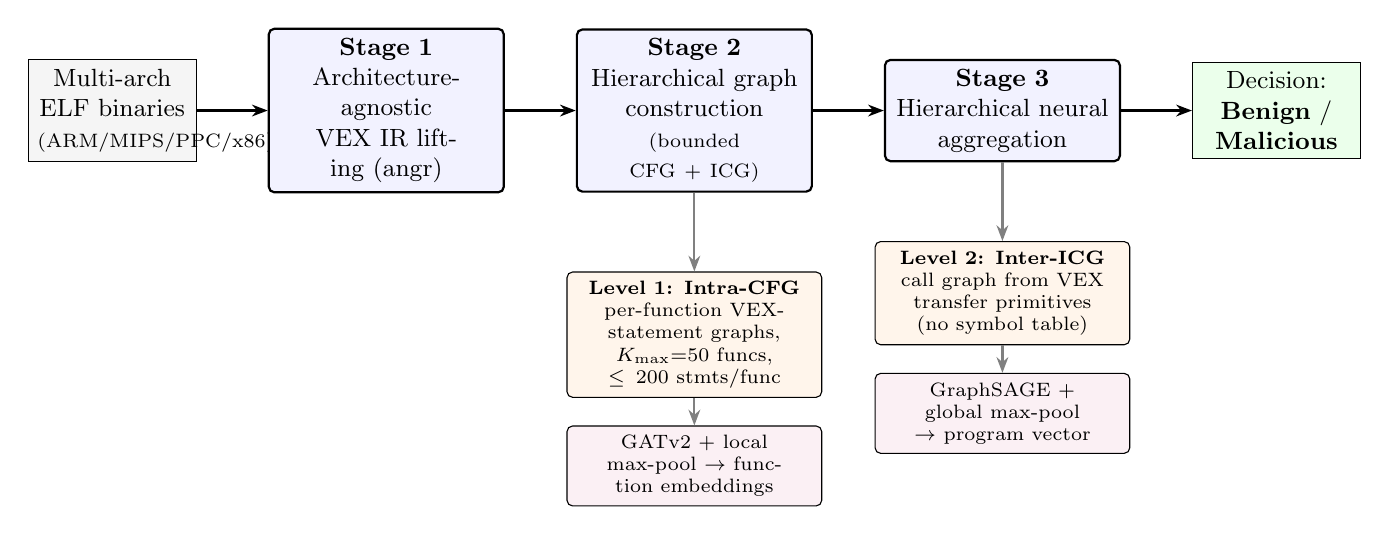
\begin{tikzpicture}[
  font=\small, >={Stealth[length=2mm]},
  stage/.style={draw, rounded corners=2pt, align=center, minimum height=1.05cm, text width=2.75cm, fill=blue!5, thick},
  io/.style={draw, align=center, minimum height=1.0cm, text width=1.9cm, fill=gray!8},
  arr/.style={->, thick},
]
\node[io] (bin) {Multi-arch\\ ELF binaries\\ \scriptsize(ARM/MIPS/PPC/x86)};
\node[stage, right=0.9cm of bin] (lift) {\textbf{Stage 1}\\ Architecture-agnostic\\ VEX~IR lifting (angr)};
\node[stage, right=0.9cm of lift] (graph) {\textbf{Stage 2}\\ Hierarchical graph\\ construction\\ \scriptsize(bounded CFG + ICG)};
\node[stage, right=0.9cm of graph] (gnn) {\textbf{Stage 3}\\ Hierarchical neural\\ aggregation};
\node[io, right=0.9cm of gnn, fill=green!8] (out) {Decision:\\ \textbf{Benign} /\\ \textbf{Malicious}};
\draw[arr] (bin) -- (lift);
\draw[arr] (lift) -- (graph);
\draw[arr] (graph) -- (gnn);
\draw[arr] (gnn) -- (out);
\node[draw, rounded corners=2pt, below=1.0cm of graph, text width=3.0cm, align=center, fill=orange!8, font=\scriptsize] (l1) {\textbf{Level 1: Intra-CFG}\\ per-function VEX-statement graphs, $K_{\max}{=}50$ funcs, $\le 200$ stmts/func};
\node[draw, rounded corners=2pt, below=1.0cm of gnn, text width=3.0cm, align=center, fill=orange!8, font=\scriptsize] (l2) {\textbf{Level 2: Inter-ICG}\\ call graph from VEX transfer primitives (no symbol table)};
\draw[arr, gray] (graph) -- (l1);
\draw[arr, gray] (gnn) -- (l2);
\node[draw, rounded corners=2pt, below=0.35cm of l1, text width=3.0cm, align=center, fill=purple!6, font=\scriptsize] (p1) {GATv2 + local max-pool $\rightarrow$ function embeddings};
\node[draw, rounded corners=2pt, below=0.35cm of l2, text width=3.0cm, align=center, fill=purple!6, font=\scriptsize] (p2) {GraphSAGE + global max-pool $\rightarrow$ program vector};
\draw[arr, gray] (l1) -- (p1);
\draw[arr, gray] (l2) -- (p2);
\end{tikzpicture}
\caption{Overview of the proposed \text{H-GNN} framework. Heterogeneous multi-architecture ELF binaries are lifted into architecture-agnostic VEX IR, decomposed into a two-level hierarchical graph (bounded intra-procedural CFGs and an inter-procedural call graph reconstructed from control-flow primitives), and encoded bottom-up with GATv2 and GraphSAGE for binary malware detection at the edge.}
\label{fig:system_overview}
\end{figure*}

\begin{enumerate}
    \item \text{Architecture-Agnostic Preprocessing Layer}: Normalizes multi-architecture binaries (ARM, MIPS, x86, PowerPC) by lifting machine instructions into a unified Intermediate Representation (VEX IR) via the \textit{angr} framework.
    \item \text{Hierarchical Graph Construction Layer}: Extracts localized Control Flow Graphs (CFGs) for individual functions under a bounded constraint to eliminate structural noise \cite{b6} (Level 1), then constructs the true Inter-procedural Call Graph to explicitly represent global functional dependencies without fragile flat sequence conversion (Level 2).
    \item Hierarchical Neural Aggregation Engine: Executes bottom-up representation learning where a local GNN function encoder processes function-level CFGs via maximum pooling, which are subsequently aggregated and refined by a global GraphSAGE processing layer and a global max-pooling readout module for final inference.
\end{enumerate}


\subsection{Threat Model and Scope}
We target static detection of cross-architecture IoT malware on resource-constrained edge gateways,
without executing samples. The adversary distributes ELF binaries cross-compiled for heterogeneous
ISAs (ARM, MIPS, PowerPC, x86), which may be stripped, statically linked, and packed (e.g., UPX), and
may undergo lightweight structural perturbation such as function insertion, reordering, or dead-code
injection. The defender inspects binary structure only. Out of scope are samples that the unpacking
stage cannot recover, heavily obfuscated or self-modifying binaries that prevent reliable lifting, and
active adversarial evasion against the model, which we identify as future work.


\subsection{Architecture-Agnostic Preprocessing and Feature Initialization}
To achieve cross-architecture compatibility, the preprocessing layer strips hardware-dependent properties prior to graph building, transforming raw machine code into platform-independent VEX IR statements \cite{b4}.

\begin{itemize}
    \item \text{Intermediate Representation Decomposition}: VEX IR abstracts away architecture-specific register layouts and instruction sets, converting complex CISC/RISC operations into side-effect-free, standardized primitives \cite{b8}. Instruction semantics are condensed into core operational behaviors such as register reads (\texttt{GET}), memory loads (\texttt{LDle}), stores (\texttt{STle}), and arithmetic operations (\texttt{Add32}).
    \item \text{Semantic Token Mapping}: Each lifted function is represented at the VEX
statement level. Every VEX statement is assigned one of a compact vocabulary of
statement tags (e.g., \texttt{WrTmp}, \texttt{Put}, \texttt{Store}, \texttt{Exit}, \texttt{LoadG}),
and each node is embedded through a trainable embedding layer $\mathbf{x} \in \mathbb{R}^{d}$
rather than a fixed one-hot vector. This yields a low-dimensional, architecture-independent
feature space learned end-to-end with the classifier.
\end{itemize}

\subsection{Hierarchical Graph Layout Construction}
To preserve localized control logic while scaling efficiently on edge platforms, H-GNN models binary software using a decoupled, dual-level hierarchical structure \cite{b6}.

\subsubsection{Level 1: Intra-procedural Control Flow Graph (CFG)}
For each isolated function $f_i$ extracted from the binary, a local Control Flow Graph is formulated as:
\begin{equation}
G_{\text{local}}^{(i)} = (V_{\text{local}}^{(i)}, E_{\text{local}}^{(i)}),
\end{equation}
where $V_{\text{local}}^{(i)}$ is the set of VEX statement nodes of function $f_i$
(each embedded from its statement tag), and $E_{\text{local}}^{(i)}$ contains both sequential
control-flow edges (within and across basic blocks) and data-dependency edges induced by VEX
temporaries.

To eliminate structural noise from redundant library routines and prevent memory explosion, we introduce a strict structural constraint $K_{\text{max}} = 50$. The local graph extraction space is bounded such that:
\begin{equation}
i \in \{1, 2, \dots, N\} \quad \text{where} \quad N = \min(\text{Num\_Functions}, K_{\text{max}}).
\end{equation}
For reproducibility, when a binary exceeds $K_{\text{max}}$ the first $K_{\text{max}}$ functions in ascending order of virtual entry address are selected. This bound limits graph size and reduces the information dilution introduced by large numbers of helper routines.

\subsubsection{Level 2: Inter-procedural Call Graph (ICG)}
To capture the macroscopic context and control transitions across separate subroutines without flattening structural dependencies, H-GNN models the global program level using the explicit execution topology of the Inter-procedural Call Graph. The global program architecture is formulated as a directed graph layout:
\begin{equation}
G_{\text{global}} = (V_{\text{global}}, E_{\text{global}}),
\end{equation}
where each functional vertex $v_i \in V_{\text{global}}$ corresponds to a dense embedding vector $\mathbf{h}^{(i)}_{f}$ representing the localized execution state of the $i$-th bounded local function CFG ($i \le N$), and each directed edge $e_{ij} \in E_{\text{global}}$ signifies an explicit inter-procedural function call interaction extracted sequentially from the binary text segment.

\subsection{Hierarchical Neural Aggregation Engine}
The network inference engine executes reasoning over the hierarchical topology via a dual-stage bottom-up aggregation process.

\subsubsection{Stage 1: Intra-Procedural Semantic Encoding}
Each bounded local CFG ($G_{\text{local}}^{(i)}$) is processed through a localized Graph Neural Network using the Graph Attention Network v2 (GATv2) architecture. The dynamic attention coefficient $\alpha_{jk}$ between two connected nodes $j$ and $k$ within the local graph is evaluated as:
\begin{equation}
\alpha_{jk} = \frac{\exp\left(\mathbf{a}^{T} \sigma\left(\mathbf{W} [\mathbf{h}_{j} \Vert \mathbf{h}_{k}]\right)\right)}{\sum_{m \in \mathcal{N}(j)} \exp\left(\mathbf{a}^{T} \sigma\left(\mathbf{W} [\mathbf{h}_{j} \Vert \mathbf{h}_{m}]\right)\right)},
\end{equation}
where $\mathcal{N}(j)$ denotes the spatial neighborhood of node $j$, $\mathbf{W}$ is a shared weight transformation matrix, $\Vert$ signifies concatenation, and $\mathbf{a}$ represents the dynamic attention weight vector. 

The updated representation of node $i$ aggregates its neighbours weighted by these
coefficients:
\begin{equation}
\mathbf{h}_{i}' = \sigma\!\left( \sum_{j \in \mathcal{N}(i)} \alpha_{ij}\, \mathbf{W}\, \mathbf{h}_{j} \right),
\end{equation}
The intra-procedural encoder stacks two GATv2 layers: the first uses multi-head attention with
concatenation, and the second uses a single attention head.

Following iterative message-passing, the updated representations are compressed into a singular function-level embedding vector $\mathbf{h}_{f}^{(i)} \in \mathbb{R}^{D}$ via an anisotropic local maximum pooling readout phase:
\begin{equation}
\mathbf{h}_{f}^{(i)} = \mathrm{ReLU}\left(\mathbf{W}_{f} \cdot \left[ \max_{v \in V_{\text{local}}^{(i)}} \mathbf{h}_{v} \right] \right),
\end{equation}
where $\mathbf{W}_{f}$ denotes the functional transformation matrix. Max-pooling preserves sparse, localized signals within a function that averaging would dilute.

\subsubsection{Stage 2: Inter-Procedural Propagation and Readout Phase}
The $N$ function embeddings are deployed onto the vertices of the Inter-procedural Call Graph to initialize the program state matrix representing the global executable distribution:
\begin{equation}
\mathbf{X}_{\text{program}} = \left[ \mathbf{h}_{f}^{(1)} \Vert \mathbf{h}_{f}^{(2)} \Vert \dots \Vert \mathbf{h}_{f}^{(N)} \right]^{T} \in \mathbb{R}^{N \times D}.
\end{equation}
To dynamically diffuse malware characteristics across function boundaries and track contextual dependencies, an inter-procedural convolution layer ($\text{GNN}_{\text{global}}$, instantiated via inductive GraphSAGE convolutions) is executed over the true call graph adjacency structure $\mathbf{A}_{\text{call}}$ extracted from the binary text segment:
\begin{equation}
\mathbf{X}_{\text{refined}} = \mathrm{ReLU}\left( \text{GNN}_{\text{global}}(\mathbf{X}_{\text{program}}, \mathbf{A}_{\text{call}}) \right).
\end{equation}
The underlying inter-procedural message passing routine at an arbitrary functional network layer $l$ is formalized as follows:
\begin{equation}
\mathbf{h}_{v_i}^{(l)} = \text{ReLU} \left( \mathbf{W}^{(l)} \cdot \left[ \mathbf{h}_{v_i}^{(l-1)} \,\|\, \text{MEAN} \left( \{ \mathbf{h}_{v_j}^{(l-1)}, \forall v_j \in \mathcal{N}(v_i) \} \right) \right] \right),
\end{equation}
where $\mathcal{N}(v_i)$ signifies the set of immediate neighboring subroutines interacting with $v_i$ within $\mathbf{A}_{\text{call}}$, and $\mathbf{W}^{(l)}$ denotes the trainable structural weight matrix.

To obtain a program-level representation, H-GNN applies global max-pooling across the refined call graph:
\begin{equation}
\mathbf{g}_{\text{program}} = \operatorname*{max}_{i=1}^{N} \mathbf{X}_{\text{refined}}[i, :].
\end{equation}
This hierarchical pooling workflow pairs local max-pooling within function blocks with global max-pooling over the inter-procedural call graph, selecting the most salient functional responses at both levels; an empirical comparison (Section~\ref{sec:ablation}) shows this outperforms global mean-pooling on our dataset. The unified representation vector $\mathbf{g}_{\text{program}}$ is then projected onto the output classification space, where the final inference probability vector $\hat{\mathbf{y}}$ is derived via a LogSoftmax activation:
\begin{equation}
\hat{\mathbf{y}} = \mathrm{LogSoftmax}\left(\mathbf{W}_{c} \mathbf{g}_{\text{program}} + \mathbf{b}_{c}\right),
\end{equation}
where $\mathbf{W}_{c}$ and $\mathbf{b}_{c}$ denote the classifier weight matrix and bias vector, mapping the structural verdict to either the benign or the malicious class.

%--------------------Experimental Results and Analysis
\section{Experimental Results and Analysis}
\label{sec:experiments}

We evaluate \text{H-GNN} on two research questions our current setup
answers directly: \textbf{RQ1} (detection performance on a
confound-controlled, cross-architecture dataset) and \textbf{RQ3} (the
contribution of each structural component). Cross-ISA generalisation
(RQ2) and on-device efficiency (RQ4) are discussed as future work in
Section~\ref{sec:conclusion}.

\subsection{Dataset and Experimental Setup}
\label{sec:setup}

A central methodological concern in cross-architecture IoT malware
detection is that benign and malicious samples often differ in build
provenance---architecture, linking, stripping, packing, and compiler
toolchain---rather than in behaviour, letting a classifier reach high
accuracy by learning artefacts instead of maliciousness. To control for
this, the benign class is compiled by the authors from open-source
software using period cross-compilation toolchains, so that its
architecture, ABI, linking, stripping, and packing distributions match
the malware class. We quantify residual leakage with a metadata-only
probe (Section~\ref{sec:threats}): on a naive benign/malware split it
reaches roughly \probeOld{} accuracy, whereas on our matched dataset it
drops to \probeNew{} once file size is excluded, indicating that low-level
build artefacts no longer separate the classes.

The dataset contains \dsTotal{} ELF binaries over six instruction-set
targets (ARM OABI/EABI, MIPS big/little endian, PowerPC, i386). Malware is
drawn from public IoT corpora, deduplicated by SHA-256, restricted to
architectures supported by our lifter, and UPX-unpacked prior to analysis;
benign samples span \dsBenignProg{} distinct open-source programs. We use a
\emph{family-/program-disjoint} split so that programs and malware
families at test time are unseen during training: \dsTrain{} training,
\dsVal{} validation, and \dsTest{} test graphs.

Each binary is lifted to VEX IR and decomposed into at most $K_{\max}=50$
bounded intra-procedural graphs, each capped at $200$ VEX statements.
Models train for $30$ epochs (Adam, lr $2\times10^{-4}$, weight decay
$10^{-4}$, batch size $8$, NLL loss); the best-validation-F1 epoch is kept
for testing. Results are mean~$\pm$~std over five seeds unless noted.

\subsection{RQ1: Detection Performance}
\label{sec:detection}

Table~\ref{tab:detection} reports test-set performance. \text{H-GNN}
attains F1 $\hgnnF{}\pm\hgnnFstd{}\%$ with PR-AUC $\hgnnPrauc{}\%$ and a
false-positive rate of $\hgnnFpr{}\%$ at $95\%$ true-positive rate. These
numbers are obtained where a metadata-only classifier is near chance once
file size is removed, so the model's decisions derive from program
structure rather than build provenance. The headline F1 is therefore an
honest measure of malicious structure under a strict, family-disjoint
protocol.

\begin{table}[t]
\centering
\caption{Detection performance of \text{H-GNN} on the family-disjoint test
set (mean $\pm$ std, five seeds).}
\label{tab:detection}
\begin{tabular}{lc}
\hline
Metric & Value (\%) \\
\hline
F1-score        & $\hgnnF \pm \hgnnFstd$ \\
Accuracy        & $\hgnnAcc \pm \hgnnAccStd$ \\
Precision       & $\hgnnPrec \pm \hgnnPrecStd$ \\
Recall          & $\hgnnRec \pm \hgnnRecStd$ \\
MCC             & $\hgnnMcc \pm \hgnnMccStd$ \\
PR-AUC          & $\hgnnPrauc \pm \hgnnPraucStd$ \\
FPR @ 95\% TPR  & $\hgnnFpr \pm \hgnnFprStd$ \\
\hline
\end{tabular}
\end{table}

\paragraph{Operational precision under class imbalance.}
Because malware is rare in deployment, we report precision under realistic
base rates rather than only the balanced test set. As malware prevalence
falls to $10\%$, $1\%$, and $0.1\%$, precision drops to $\brTen$, $\brOne$,
and $\brTenth$ respectively, reflecting the base-rate effect inherent to
rare-event detection. We state this explicitly so that the required
operating point for gateway deployment (e.g.\ pairing \text{H-GNN} with a
lightweight pre-filter to raise effective prevalence) is clear rather than
obscured by a balanced-set figure.

\subsection{RQ3: Ablation Study}
\label{sec:ablation}

We retrain \text{H-GNN} with individual components removed under the same
protocol (Table~\ref{tab:ablation}, Fig.~\ref{fig:ablation_study}).

\begin{table}[t]
\centering
\caption{Component ablation (test F1). Removing the hierarchical
decomposition causes the largest degradation. The no-hierarchy row is the
mean of two seeds.}
\label{tab:ablation}
\begin{tabular}{lc}
\hline
Configuration & F1 (\%) \\
\hline
\text{H-GNN} (full, global max-pool)          & $\hgnnF \pm \hgnnFstd$ \\
\quad global max-pool $\rightarrow$ mean-pool & $\ablMean \pm \ablMeanStd$ \\
\quad w/o hierarchical decomposition          & $\ablNoHier$ \\
\hline
\end{tabular}
\end{table}

\begin{figure}[!t]
\centering
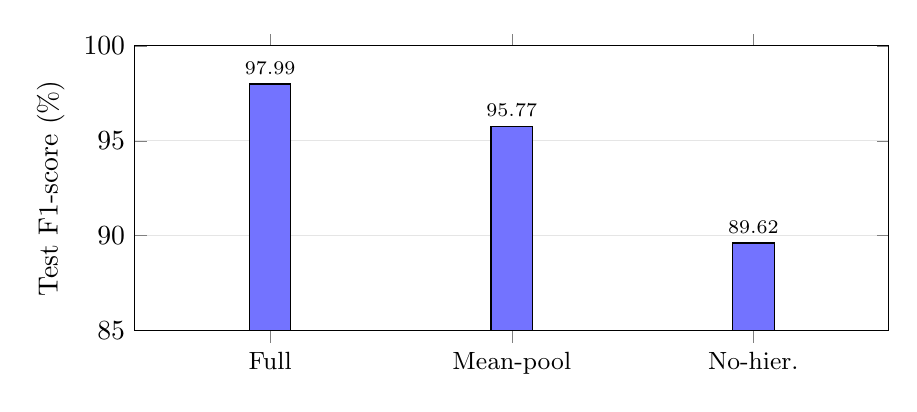
\begin{tikzpicture}
\begin{axis}[
  ybar, width=0.92\columnwidth, height=5.2cm, bar width=15pt,
  ymin=85, ymax=100, ylabel={Test F1-score (\%)},
  symbolic x coords={Full, {Mean-pool}, {No-hier.}}, xtick=data,
  x tick label style={font=\small}, nodes near coords,
  nodes near coords style={font=\scriptsize, /pgf/number format/precision=2, /pgf/number format/fixed},
  enlarge x limits=0.28, ymajorgrids=true, grid style=gray!20,
]
\addplot[fill=blue!55] coordinates {(Full,97.99) ({Mean-pool},95.77) ({No-hier.},89.62)};
\end{axis}
\end{tikzpicture}
\caption{Component ablation (test F1-score). The full \text{H-GNN} with hierarchical decomposition and global max-pooling attains \hgnnF\%; replacing global max-pooling with mean-pooling drops it to \ablMean\%, and removing the hierarchical decomposition drops it to \ablNoHier\% (mean of two seeds), confirming both design choices.}
\label{fig:ablation_study}
\end{figure}


Two findings emerge. First, collapsing the two-level hierarchy into a
single flat graph reduces F1 from $\hgnnF\%$ to $\ablNoHier\%$
(about $8$ points), confirming that separating intra-procedural semantics
from inter-procedural structure is the dominant contributor. Second,
replacing global max-pooling with mean-pooling reduces F1 to $\ablMean\%$,
indicating that selecting the most salient functional responses is more
effective than averaging them here; we adopt global max-pooling in the
final model.


\section{Threats to Validity}
\label{sec:threats}

\textbf{Construct validity.} A key risk in cross-architecture malware datasets is that benign and
malicious samples differ in build provenance (architecture, linking, stripping, packing, compiler)
rather than in behaviour, allowing a classifier to exploit these artefacts. To control this, we
construct a benign set whose architecture, ABI, linking, stripping, and packing distributions are
matched to the malware set, and quantify residual leakage with a metadata-only probe. On a naive
benign/malware split the probe reaches roughly \hgnnProbeOld\ accuracy, whereas on our matched dataset
it drops to \hgnnProbeNoSize\ once file size is excluded, indicating that architecture, linking,
stripping, and packing no longer separate the classes. Residual file-size differences are handled at
the model level: H-GNN operates on CFG structure, and the $K_{\max}$ bound limits graph size; an
ablation confirms the model does not rely on raw size.

\textbf{Internal validity.} To avoid train/test leakage from near-duplicate malware variants and
shared benign programs, we deduplicate by SHA-256 and evaluate under a family-/program-disjoint split,
where test programs and malware families are unseen during training.

\textbf{External validity.} The benign set is assembled from a finite set of open-source programs and
two toolchain generations; it may not capture all legitimate IoT software. We report the number of
distinct benign programs and include both period and modern toolchains to mitigate compiler-era bias.

\textbf{Conclusion validity.} Results are reported across multiple random seeds; we use group-aware
cross-validation and report mean and standard deviation to reduce sensitivity to a single partition.

%-----------------Ket luan---------------------
\section{Conclusion and Future Work}
\label{sec:conclusion}

We introduced \method{}, a hierarchical GNN framework for cross-architecture
IoT malware detection that couples intra-functional VEX-IR CFG semantics
with an explicit inter-procedural call graph, enabling compiler-agnostic
threat identification across heterogeneous ISAs.
Experimental evaluations on a confound-controlled, family-disjoint
dataset confirm that \method{} achieves an F1-score of $\hgnnF\%$, with
ablation studies confirming the necessity of each hierarchical component.

Moving forward, we envision several promising directions for future exploration:
\begin{itemize}
    \item \text{Limitations:} \method{} currently assumes that \textit{angr}
    can successfully lift the target binary; heavily packed or self-modifying
    binaries may require an unpacking pre-stage before analysis.
    \item \text{Scalability and Latency Optimization:} We aim to integrate
    graph sparsification and sub-graph partitioning techniques to reduce
    computational overhead in high-throughput enterprise environments.
    \item \text{Adversarial Graph Resilience:} We will investigate defensive
    training against graph evasion tactics such as dead-code injection,
    function splitting, and control-flow obfuscation.
    \item \text{Explainable AI (XAI) for Threat Intelligence:} We intend
    to embed explainability frameworks (\textit{e.g.}, GNNExplainer) to help
    analysts localize malicious sub-graphs and convert neural predictions into
    actionable cyber threat intelligence.
\end{itemize}


\section*{Data and Code Availability}
Our source code and dataset manifest --- including the SHA-256 hash of every sample and the exact
train/validation/test partition --- are available in a public repository (URL provided upon acceptance). For safety, malware binaries
are not redistributed; only their hashes are released so the evaluation set can be reconstructed from
public malware repositories. The benign set is compiled by the authors from open-source software, and
the build scripts are included.


\vspace{-4pt}
\begin{thebibliography}{10}

\bibitem{b1}
O.~Alrawi, C.~Lever, K.~Valakuzhy, R.~Court, K.~Snow, F.~Monrose, and M.~Antonakakis, ``The circle of life: A large-scale study of the {IoT} malware lifecycle,'' in {\em Proc. USENIX Security Symposium}, 2021, pp.~3505--3522.

\bibitem{b2}
R.~Roman, J.~Lopez, and M.~Mambo, ``Mobile edge computing, fog et al.: A survey and analysis of security threats and challenges,'' {\em Future Generation Computer Systems}, vol.~78, pp.~680--698, 2018.

\bibitem{b3}
E.~Cozzi, M.~Graziano, Y.~Fratantonio, and D.~Balzarotti, ``Understanding {Linux} malware,'' in {\em IEEE Symposium on Security and Privacy (SP)}, 2018, pp.~161--175.

\bibitem{b4}
Y.~Kawakoya, S.~Akabane, M.~Iwamura, and T.~Okamoto, ``{Xunpack}: Cross-architecture unpacking for {Linux} {IoT} malware,'' in {\em Proc. International Symposium on Research in Attacks, Intrusions and Defenses (RAID)}, 2023, pp.~471--484.


\bibitem{b5}
R.~Chaganti, V.~Ravi, and T.~D. Pham, ``Deep learning based cross architecture internet of things malware detection and classification,'' {\em Computers \& Security}, vol.~120, p.~102779, 2022.

\bibitem{b6}
A.~Abusnaina, A.~Khormali, H.~Alasmary, J.~Park, A.~Anwar, and A.~Mohaisen, ``Adversarial learning attacks on graph-based {IoT} malware detection systems,'' in {\em Proc. IEEE International Conference on Distributed Computing Systems (ICDCS)}, 2019, pp.~1296--1305.


\bibitem{b7} Y. Pa, S. Suzuki, K. Yoshioka, T. Matsumoto, T. Kasama, and C. Rossow, ``IoTPOT: A Novel Honeypot for Revealing Current IoT Threats,'' \textit{Journal of Information Processing}, vol. 24, no. 3, pp. 522--533, 2016. doi: 10.2197/ipsjjip.24.522.

\bibitem{b8}
X.~Xu, C.~Liu, Q.~Feng, H.~Yin, L.~Song, and D.~Song, ``Neural network-based graph embedding for cross-platform binary code similarity detection,'' in {\em Proc. ACM SIGSAC Conference on Computer and Communications Security (CCS)}, 2017, pp.~363--376.

\bibitem{b9}
Y.~Duan, X.~Li, J.~Wang, and H.~Yin, ``{DeepBinDiff}: Learning program-wide code representations for binary diffing,'' in {\em Proc. Network and Distributed System Security Symposium (NDSS)}, 2020.

\bibitem{b10}
Z.~Luo \textit{et al.}, ``{VulHawk}: Cross-architecture vulnerability
detection with entropy-based binary code search,''
in {\em Proc. Network and Distributed System Security Symposium (NDSS)}, 2023.

\bibitem{malgraph2022}
X.~Ling, L.~Wu, W.~Deng, Z.~Qu, J.~Zhang, S.~Zhang, T.~Ma, B.~Wang, C.~Wu, and S.~Ji,
``{MalGraph}: Hierarchical Graph Neural Networks for Robust {Windows} Malware Detection,''
in \emph{Proc. IEEE INFOCOM}, 2022, pp.~1998--2007,
doi: 10.1109/INFOCOM48880.2022.9796786.

\bibitem{wang2021hier}
S.~Wang, Y.~Zhao, G.~Liu, and B.~Su,
``A Hierarchical Graph-Based Neural Network for Malware Classification,''
in \emph{Neural Information Processing (ICONIP 2021)},
LNCS, vol.~13111, 2021, pp.~621--633,
doi: 10.1007/978-3-030-92273-3\_51.

\end{thebibliography}


\end{document}